\documentclass[11pt,oneside,a4paper]{article}
\usepackage{graphicx}
\usepackage{booktabs}
\usepackage{caption}
\usepackage{subcaption}
\usepackage{amsmath}
\usepackage{amsfonts}
\usepackage{amssymb}
\usepackage{lscape}
\usepackage{psfrag}
\usepackage[usenames]{color}
\usepackage{bbm}
\usepackage[update]{epstopdf}
\usepackage[bookmarks,pdfstartview=FitH,a4paper,pdfborder={0 0 0}]{hyperref}
\usepackage{verbatim}
\usepackage{listings}
\usepackage{textcomp}
\usepackage{course}
\usepackage{fancyhdr}
\usepackage{multirow}
\pagestyle{fancy}
\usepackage{tikz}
\usepackage{subcaption} 

\renewcommand{\sectionmark}[1]{\markboth{#1}{#1}}
\renewcommand{\subsectionmark}[1]{\markright{#1}}

\fancyhf{}
\fancyhead[RO]{\nouppercase{\footnotesize\sc\leftmark\ \hrulefill\ \thepage}}
\fancyhead[RE]{\nouppercase{\footnotesize\sc\thepage\ \hrulefill\ }}
\renewcommand{\headrulewidth}{0pt}

\makeatletter
\def\cleardoublepage{\clearpage\if@twoside \ifodd\c@page\else%
\hbox{}%
\thispagestyle{empty}%
\clearpage%
\if@twocolumn\hbox{}\clearpage\fi\fi\fi}
\makeatother


\renewcommand{\topfraction}{0.9}  % max fraction of floats at top
\renewcommand{\bottomfraction}{0.8} % max fraction of floats at bottom
% Parameters for TEXT pages (not float pages):
\setcounter{topnumber}{2}
\setcounter{bottomnumber}{2}
\setcounter{totalnumber}{4}            % 2 may work better
\setcounter{dbltopnumber}{2}           % for 2-column pages
\renewcommand{\dbltopfraction}{0.9}    % fit big float above 2-col. text
\renewcommand{\textfraction}{0.07}     % allow minimal text w. figs
% Parameters for FLOAT pages (not text pages):
\renewcommand{\floatpagefraction}{0.7}  % require fuller float pages
% N.B.: floatpagefraction MUST be less than topfraction !!
\renewcommand{\dblfloatpagefraction}{0.7} % require fuller float pages

\sloppy

\widowpenalty=10000
\clubpenalty=10000

\edef\today{%\number\day\
\ifcase\month\or
January\or February\or March\or April\or May\or June\or July\or
August\or September\or October\or November\or December\fi\ \number\year}
\title{\vspace*{40.0mm}
  \bf\sf Support Vector Machine Assignment 
         \vspace*{20.0mm} \\
  \vspace*{40.0mm}
  %\vspace{-20mm}\framebox{DRAFT VERSION}\vspace{20mm} \\
  }
\author{\sf Mohamedhakim Elakhrass}
\date{\sf 15/07/2016}

\begin{document}

\begin{figure}
  \parbox[t]{125mm}{
    \vspace*{6mm}
    \scriptsize\sf           FACULTY OF BIOSCIENCE ENGINEERING\\
    \scriptsize\sf           Masters of Bioinformatics \\
    \scriptsize\sf\bfseries  Support Vector Machines \\}
  \parbox[t]{40mm}{
    \begin{flushright}
      \includegraphics[height=15mm]{logo.eps}
    \end{flushright}}
\end{figure}

\maketitle
\thispagestyle{empty}
\raggedbottom

\cleardoublepage
\pagenumbering{roman}
\setcounter{tocdepth}{2}
\tableofcontents
\cleardoublepage
\pagenumbering{arabic}

\cleardoublepage

\section{Objectives}
The objectives of this assignment are to learn and work with real life applications of SVM. 
\section{Simple 2 Gaussian}
This sections looks at two simulated datasets. The datasets are created using the MatLab $randn()$ function. One dataset is centered around (1,1) and the other (-1,1)\\

\begin{figure}[h!]
	\setbox0\hbox{%
		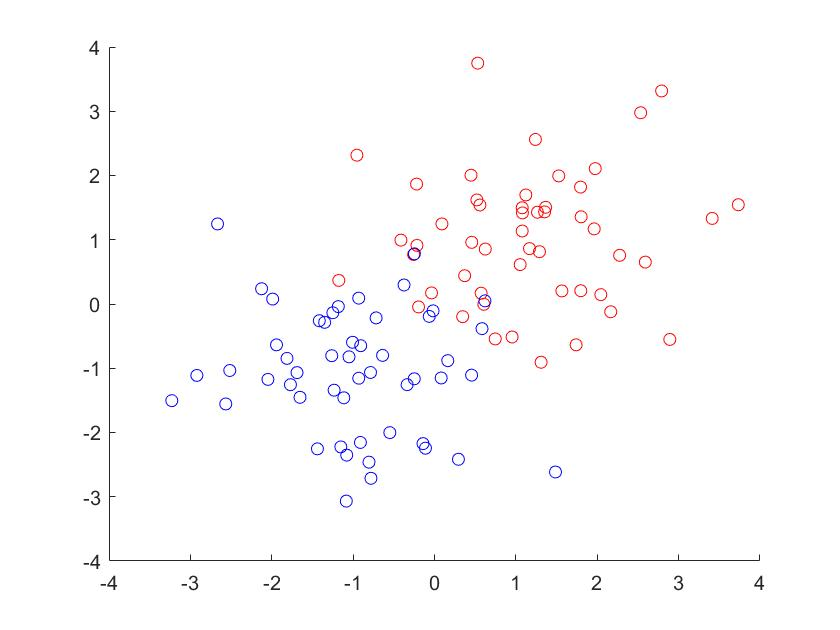
\includegraphics[width=.45\textwidth]{../Figures/2_Gaussians}%
	}%
	\setbox2\hbox{%
		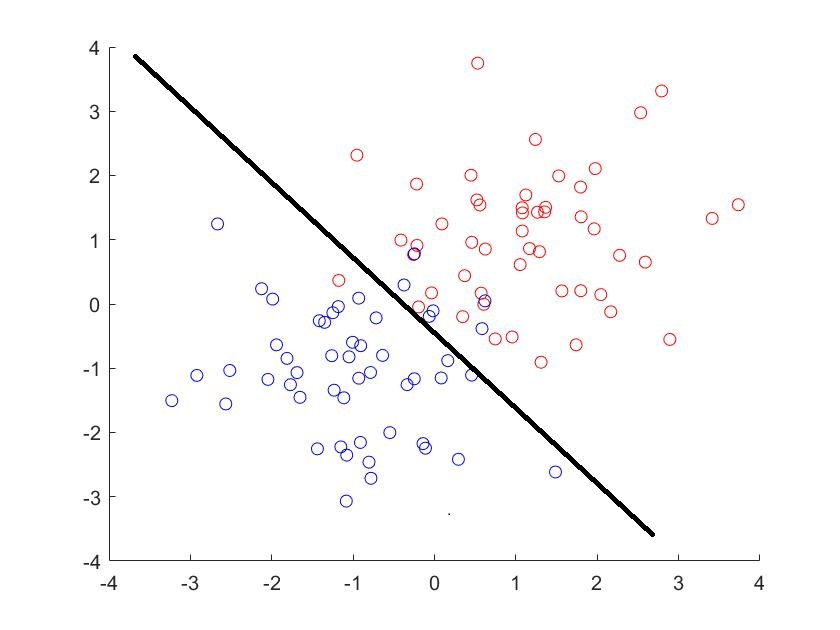
\includegraphics[width=.45\textwidth]{../Figures/2_Gaussians_with_classifier}%
	}%
	\ifdim\ht0>\ht2
	\setbox0\hbox{%
		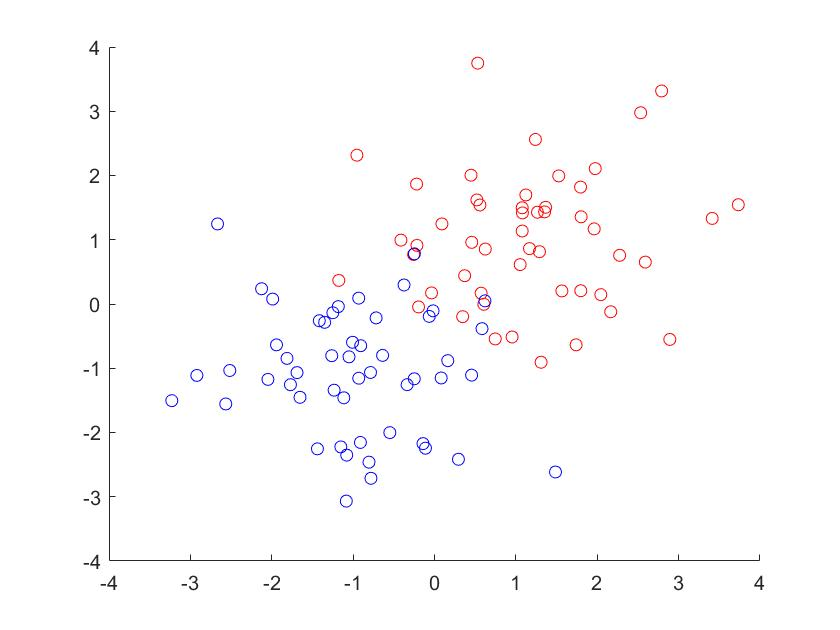
\includegraphics[height=\ht2]{../Figures/2_Gaussians}%
	}%
	\else
	\setbox2\hbox{%
		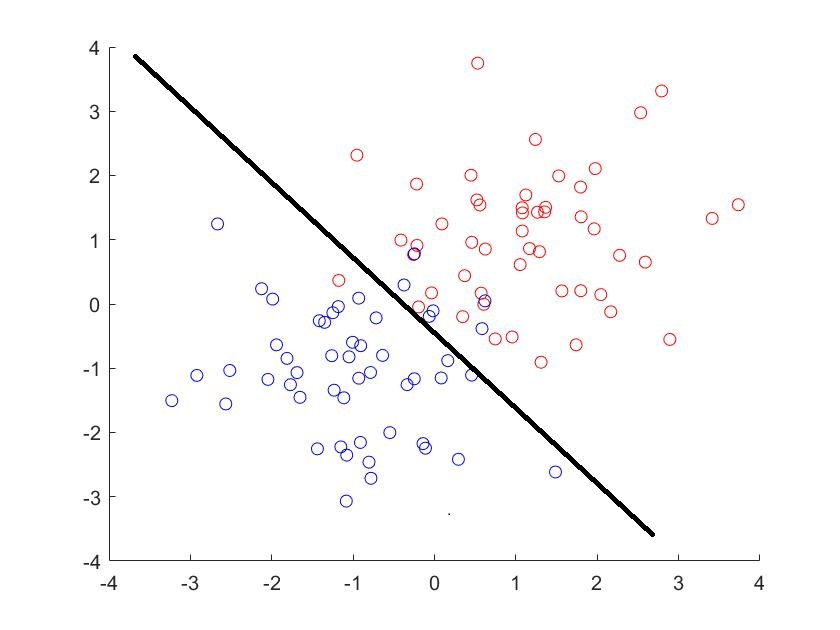
\includegraphics[height=\ht0]{../Figures/2_Gaussians_with_classifier}%
	}%
	\fi
	\noindent
	\parbox{.45\textwidth}{%
		\centering
		\unhbox0
		\caption{Two Simulated Datasets.}
	}%
	\hfil
	\parbox{.45\textwidth}{%
		\centering
		\unhbox2
		\caption{Two Simulated Datasets with Optimal Classifier.}
	}%
\end{figure}




\textbf{Given this figure, can you make a geometric construction using lines to estimate the optimal classifier? Under which conditions do you think this construction is optimal/valid?}\\

Figure 1:a is the output of the simulated datasets. As shown in figure 1:b it is possible to show an optimal classifier. This classifier is known as the Bayes Classifier. A test observation is assigned with predictor vector $x_{0}$ to the class j for which    \[ Pr(Y=j|X=x_{0}) \] is largest. The classifier is optimal because it produces the lowest possible error rate and allows for some overlap. The classifier is valid because the underlying distribution of the dataset is known. This falls into the special case $\Sigma_{xx1} = \Sigma_{xx2} - \Sigma_{xx}$, the covariance matrices are equal and the decision boundary is linear.
\section{The Support Vector Machine}

This section will deal with an online demo of a linear and none linear SVM. It will be used to learn the intuition behind changing SVM parameters and changes in the dataset.\\


\begin{figure}[h!]
	\setbox0\hbox{%
		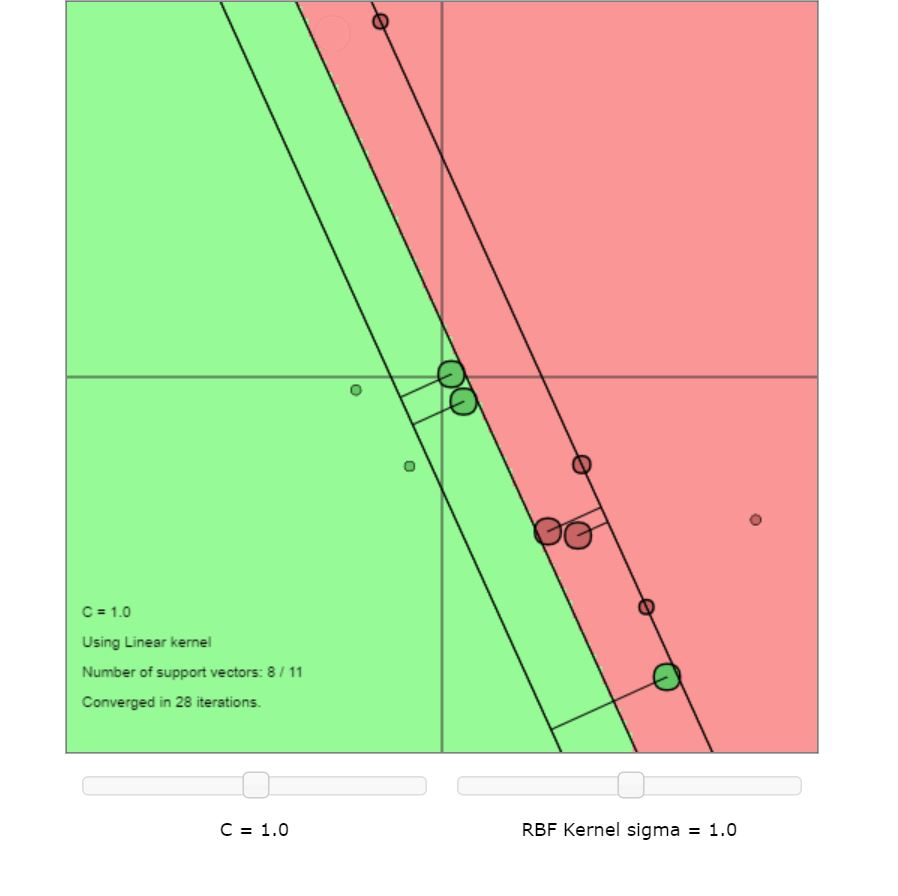
\includegraphics[width=.45\textwidth]{../Figures/Default_Linear_Kernal}%
	}%
	\setbox2\hbox{%
		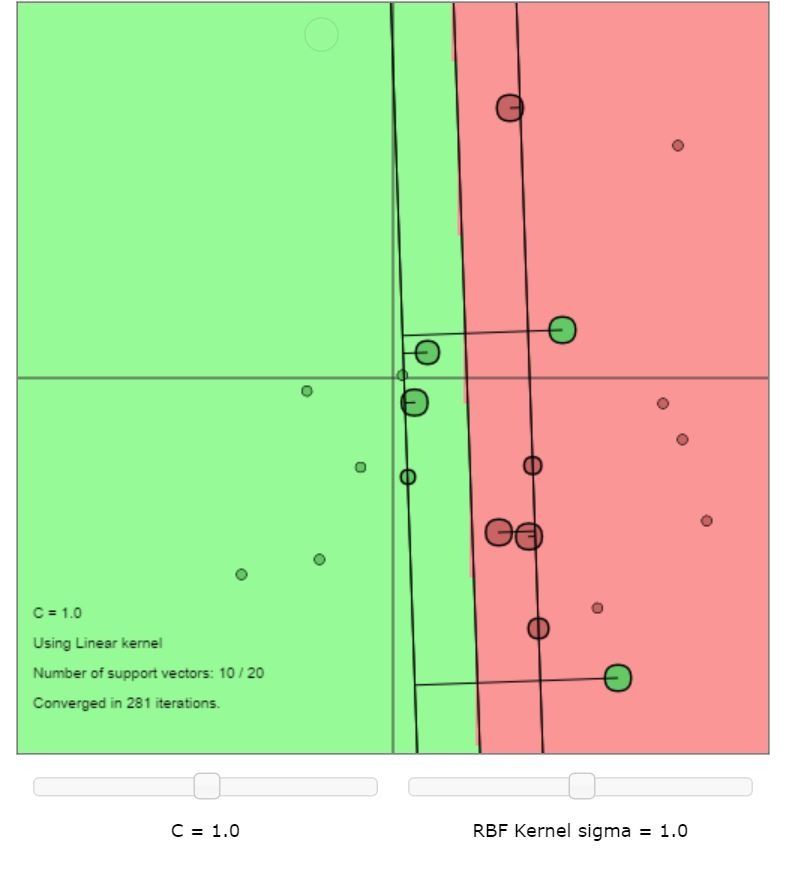
\includegraphics[width=.45\textwidth]{../Figures/10_point_linear_Kernal}%
	}%
	\ifdim\ht0>\ht2
	\setbox0\hbox{%
		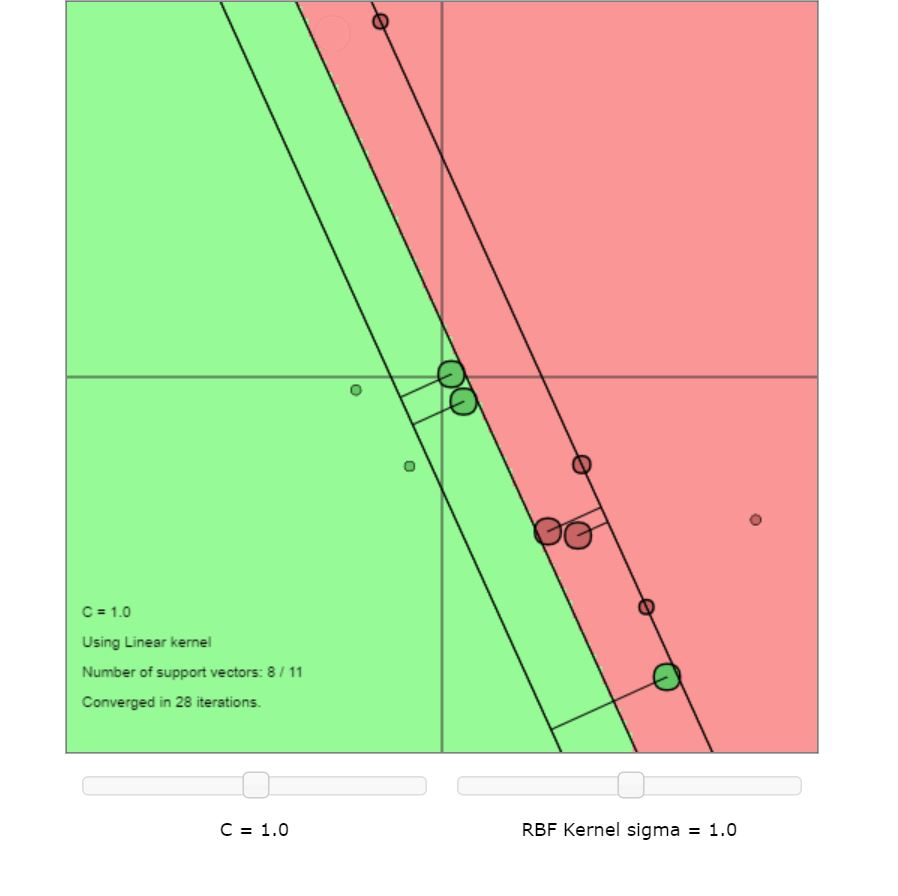
\includegraphics[height=\ht2]{../Figures/Default_Linear_Kernal}%
	}%
	\else
	\setbox2\hbox{%
		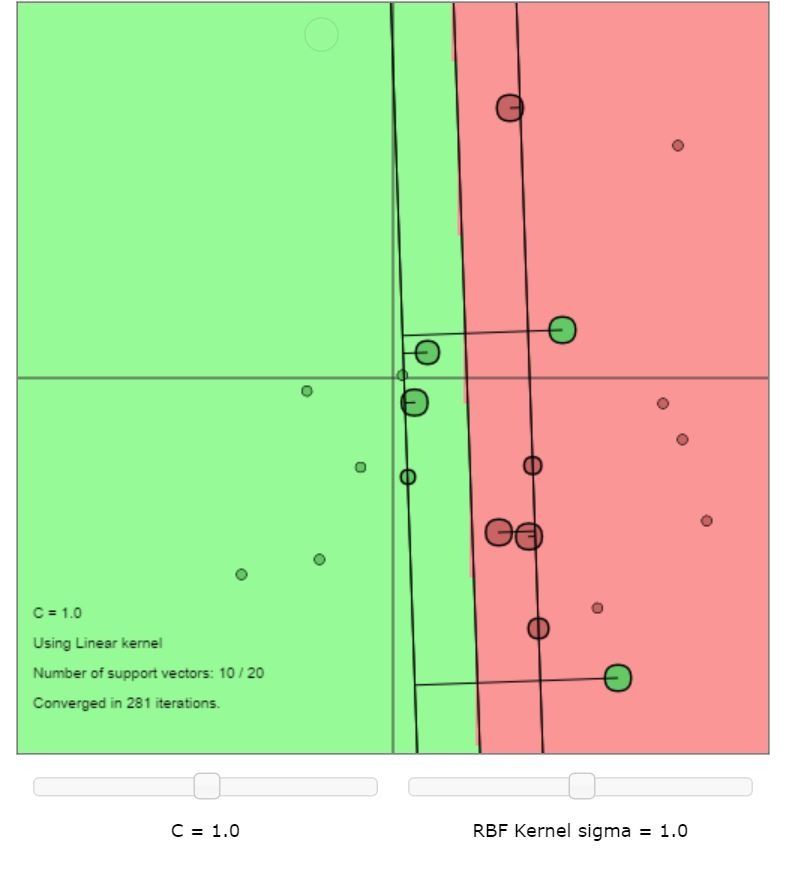
\includegraphics[height=\ht0]{../Figures/10_point_linear_Kernal}%
	}%
	\fi
	\noindent
	\parbox{.45\textwidth}{%
		\centering
		\unhbox0
		\caption{Default Linear Kernal.}
	}%
	\hfil
	\parbox{.45\textwidth}{%
		\centering
		\unhbox2
		\caption{10 Data Point Linear Kernal.}
	}%
\end{figure}

\textbf{Adjust the existing datasets to have at least 10 data points for each class. What do you observe when you are adding data points to the classes? How drastically can classification boundaries change.}

Data points added inside the margin drastically change the decision boundary  and become support vectors. Data points added to the side of the opposing color are also automatically support vectors but remain misclassified. Data points added to the same side as its own color have very little effect on the decision boundary, although the closer to the boundary the larger the effect. 

\textbf{What if you add an outlying datapoint which lies on the wrong side of the classification boundary? How does it affect the classification hyperplane?}

\begin{figure}[h!]
	 \centering
	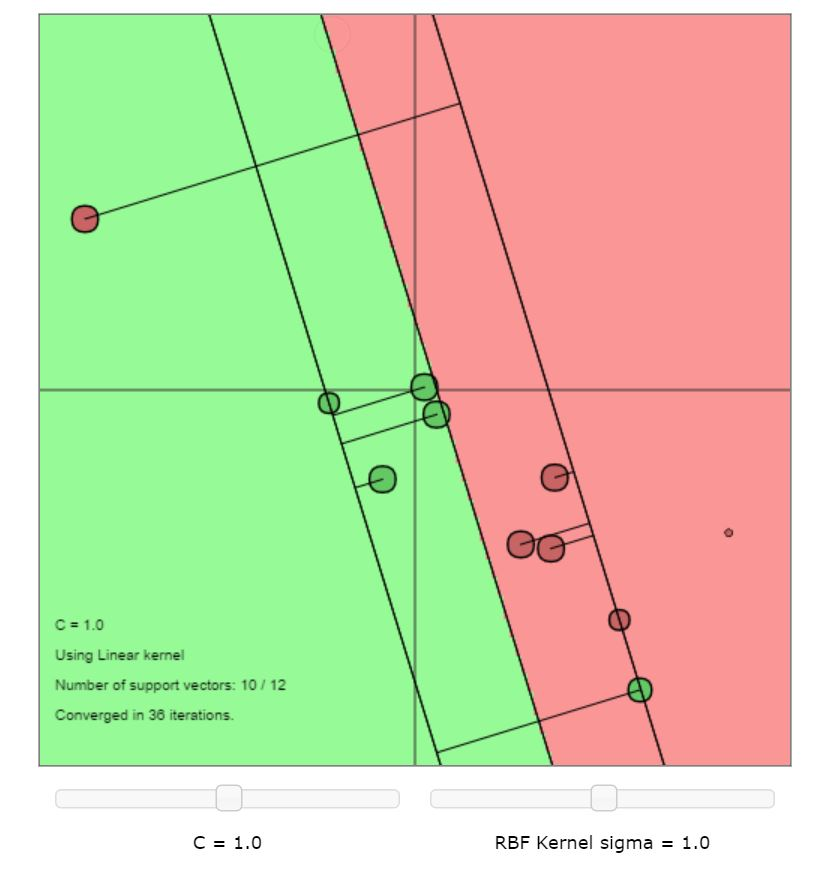
\includegraphics[scale=0.5]{../Figures/misclassified_linear_kernal}
	\caption{Outlier data point}
\end{figure}

A data point added to the wrong side of the boundary changes the direction of the hyperplane towards that point. If too many points are added the classifier misclassified all points of the opposing class. 

\textbf{Try different values of C regularization hyperparameter. How does it affect the classification outcome? What is the role of it?}\\
Using the intial dataset the effects of the regularization hyperparemter can be seen. The parameter control the slack of the SVM model. When C is high there is less tolerance for misclassification and therefore a smaller margin. When C is large there is higher tolerance for misclassification and a larger margin.

\begin{figure}[h!]
	\setbox0\hbox{%
		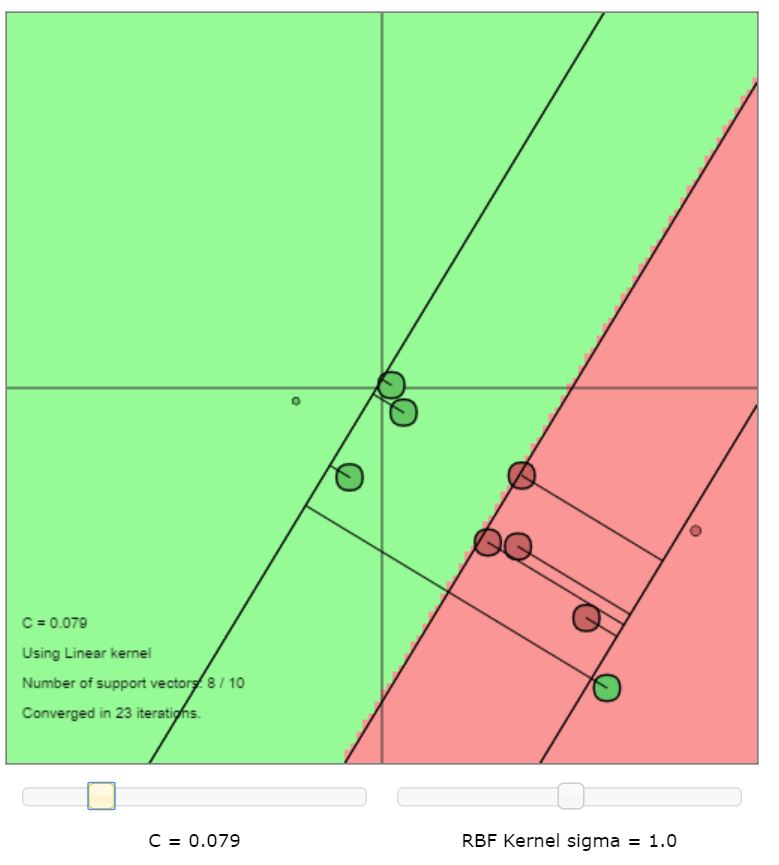
\includegraphics[width=.45\textwidth]{../Figures/small_C_linear_Kernal}%
	}%
	\setbox2\hbox{%
		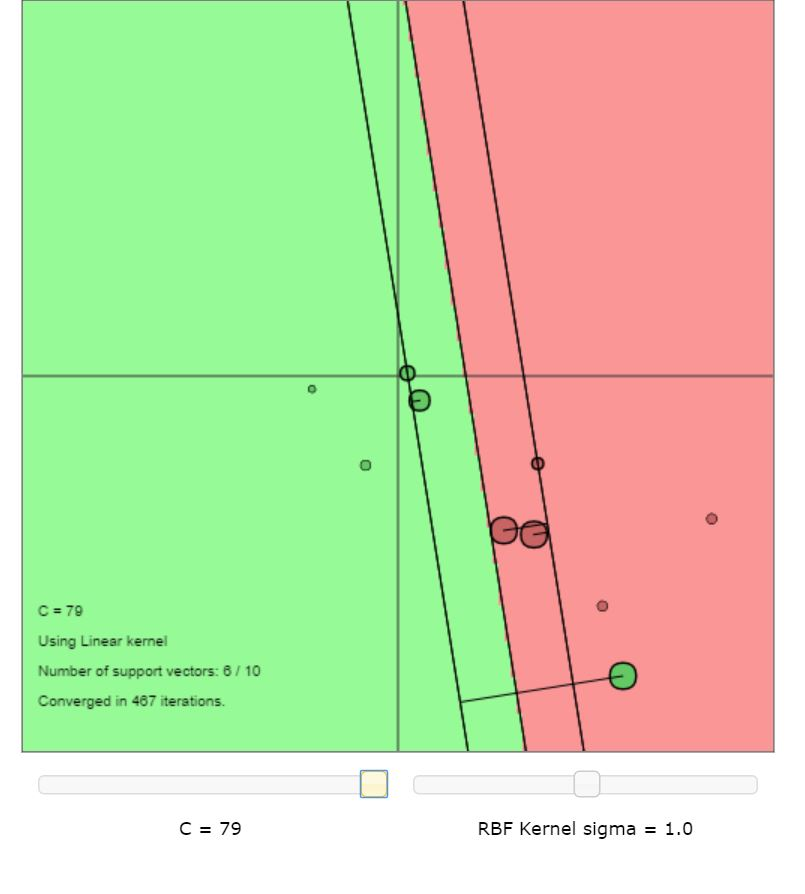
\includegraphics[width=.45\textwidth]{../Figures/large_C_linear_kernal}%
	}%
	\ifdim\ht0>\ht2
	\setbox0\hbox{%
		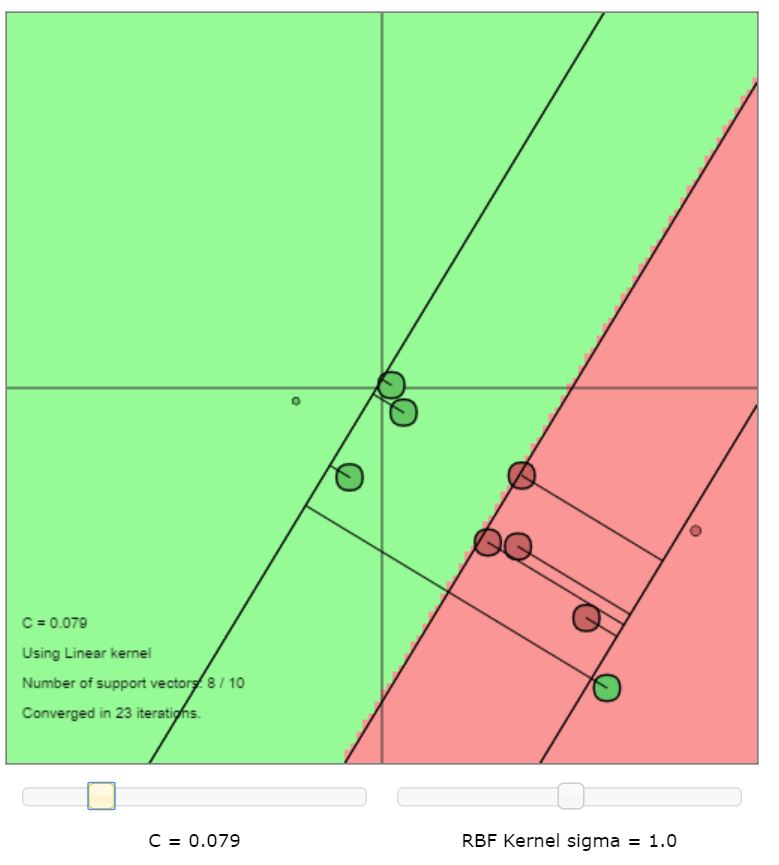
\includegraphics[height= \ht2]{../Figures/small_C_linear_Kernal}%
	}%
	\else
	\setbox2\hbox{%
		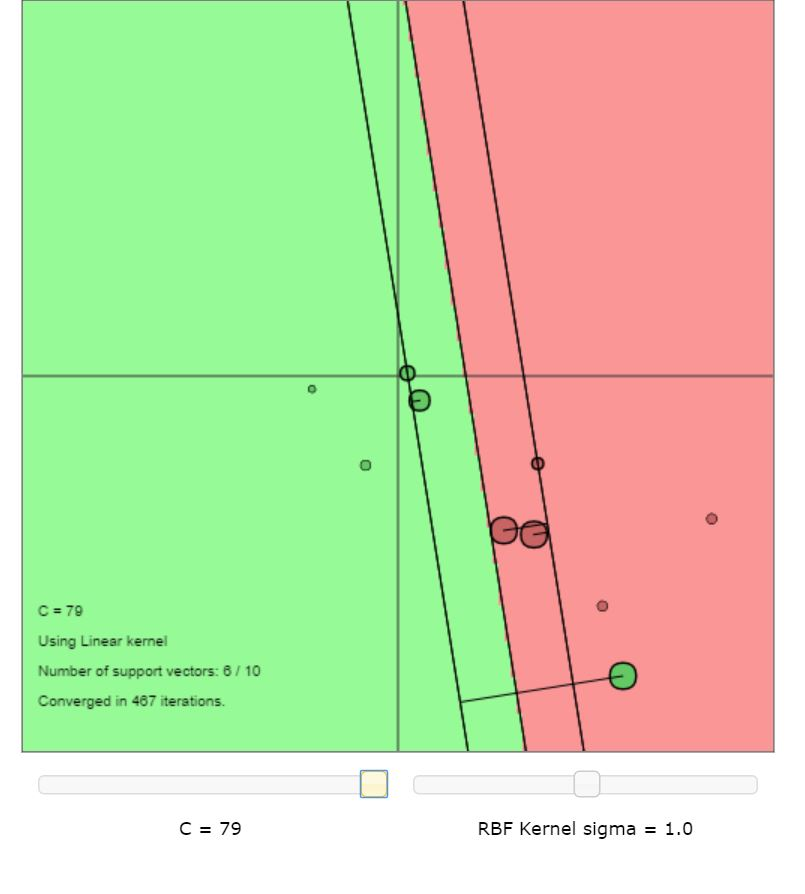
\includegraphics[height=\ht0]{../Figures/large_C_linear_kernal}%
	}%
	\fi
	\noindent
	\parbox{.45\textwidth}{%
		\centering
		\unhbox0
		\caption{C = .079}
		\label{fg:methods}
	}%
	\hfil
	\parbox{.45\textwidth}{%
		\centering
		\unhbox2
		\caption{C = 79}
		\label{fg:method_detail}
	}%
\end{figure}

 

 \begin{figure}[H]
 	\centering
 	\begin{subfigure}[b]{.5\textwidth}
 	
 		\textbf{Follow the instructions and switch back to RBF kernel by toggling the “k” button. Compare to the classification outcome of the linear case.}
 		In this section, we were asked to switch away from a linear kernel and
 		opt for the Radial Basis Function kernel (RBF). RBF are localized
 		function, centered at a particular value, and use a gaussian fit with
 		a certain spread around the center. 
 		
 		The same dataset as defined above can be seen on the graphics on
 		the right. Here, one can observe that all points have been
 		correctly classified, but the area defined are very wobbly,
 		displaying clear signs of overfitting.  
 		
 		This can be tuned by changing the value of $\sigma$, which
 		controls the bandwidth of the gaussian function, see figure
 		\ref{fig:RBF_sigma}. Larger values of $\sigma$ leading to more
 		linear decision boundaries.
 	\end{subfigure}%
 	\begin{subfigure}{.5\textwidth}
 		\vspace{-185pt}
 		\centering
 		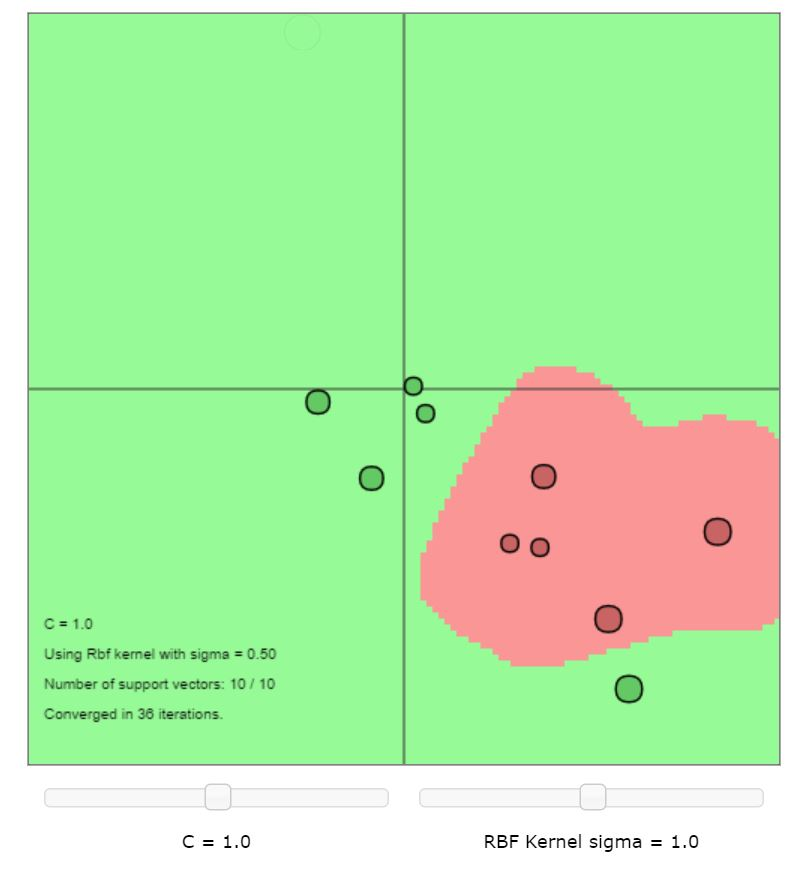
\includegraphics[width=0.9\linewidth]{../Figures/Default_RBF}
 		%\caption{RBF kernel}
 		%\label{fig:RBF_kernel}
 	\end{subfigure}
 \end{figure}
 
 \begin{figure}[h!]
 	\centering
 	\begin{subfigure}{.25\textwidth}
 		\centering
 		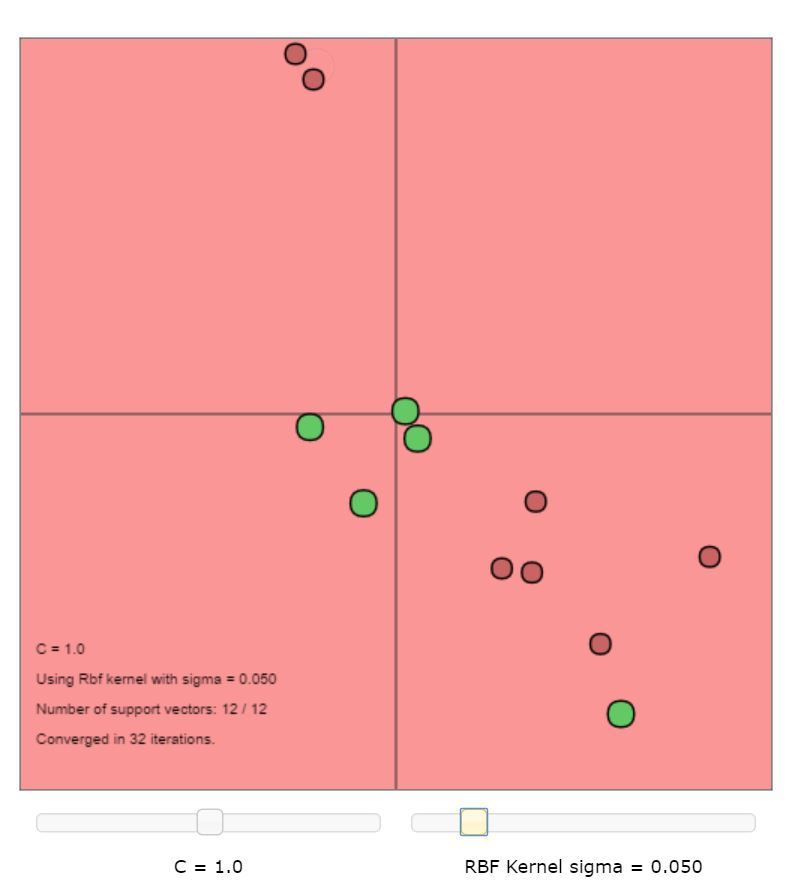
\includegraphics[width=0.9\linewidth]{../Figures/RBF_sigma_0.050}
 		\caption{Value of $\sigma = 0.050$}
 		\label{fig:rbfs1}
 	\end{subfigure}%
 	\begin{subfigure}{.25\textwidth}
 		\centering
 		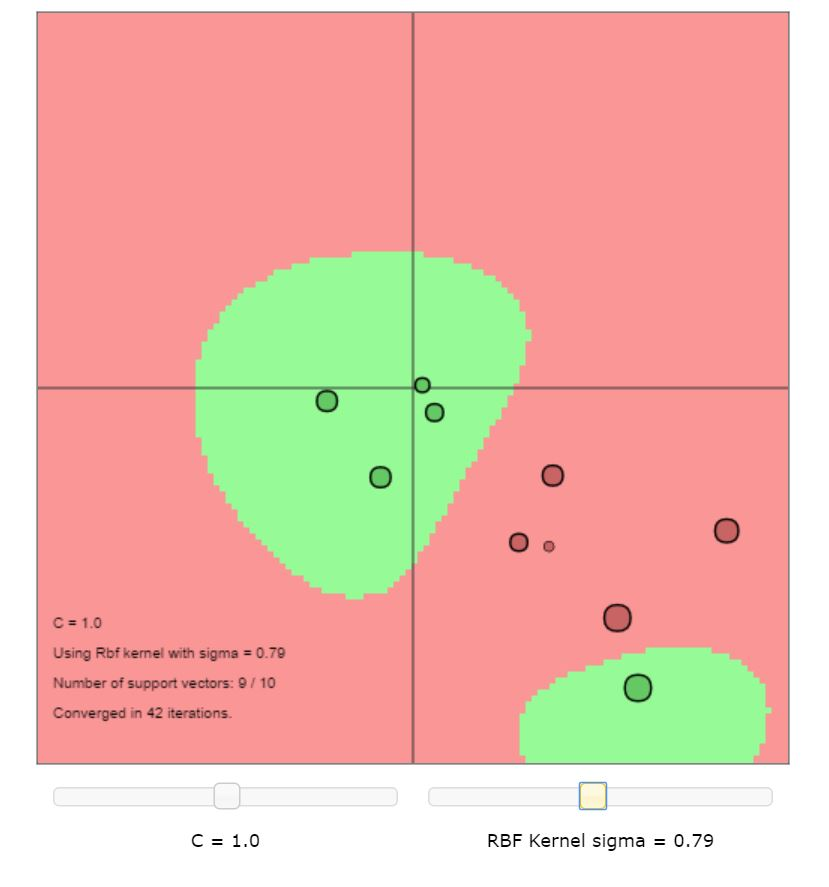
\includegraphics[width=0.9\linewidth]{../Figures/RBF_sigma_79}
 		\caption{Value of $\sigma = 1$}
 		\label{fig:rbfs2}
 	\end{subfigure}%
 	\begin{subfigure}{.25\textwidth}
 		\centering
 		\includegraphics[width=0.9\linewidth]{1-2-1-kernel_ssigma4.png}
 		\caption{Value of $\sigma = 4$}
 		\label{fig:rbfs3}
 	\end{subfigure}%
 	\begin{subfigure}{.25\textwidth}
 		\centering
 		\includegraphics[width=0.9\linewidth]{1-2-1-kernel_ssigma100.png}
 		\caption{Value of $\sigma = 100$}
 		\label{fig:rfbs4}
 	\end{subfigure}
 	\caption{Impact of $\sigma$ on the RBF classifier boundaries (C=1.0)}
 	\label{fig:RBF_sigma}
 \end{figure}

 The RBF kernal has no misclassification as opposed to the linear classifier. This is because the data set is not linearly seperable. The RBF kernal as the ability to wrap around the data.The RBF is a localized funtcion
 

\end{document}